% !TEX output_directory=output
\documentclass{beamer}

% TODO
% * clean up figures, especially handwritten ones
% * Minimize text in slides
% * Make slides stand alone (provide enough information to get gist)
% * Make it simple (e.g. “higher is better in this plot”, “reward of 4 means 0.9999”)



\usepackage[beamer]{kaufman}

\bibliography{../refs.bib}
\graphicspath{{../graphics/}}

\title{Using Reinforcement Learning for Quantum Control in Magnetic Resonance [DRAFT]}
\author{Will Kaufman}
\date{March 19, 2021}
\institute{Ramanathan Group \\ Dartmouth College}

\titlegraphic{\includegraphics[height=.1\textheight]{LonePine.pdf}}

\begin{document}

\frame{\titlepage}

\begin{frame}
\frametitle{Table of Contents}
\tableofcontents
\end{frame}

\section{Quantum control}

\begin{frame}{Quantum control in spin systems}

\begin{equation*}
    H(t) = H_\text{system} + H_\text{control}(t)
\end{equation*}

\begin{align*}
    H_\text{system} &= \sum_i \delta_i I_z^i + \sum_{i,j} d_{ij} \left( 3I_z^iI_z^j - \mathbf{I^i} \cdot \mathbf{I^j} \right) \\
        &= H_\text{CS} + H_\text{D}
\end{align*}

\begin{equation*}
    H_\text{control}(t) = -B_1(t) \sum_i \gamma_n^i I_x^i -B_2(t) \sum_i \gamma_n^i I_y^i
\end{equation*}

Can use $H_\text{control}(t)$ to achieve desired state $\rho(t)$ or dynamics $U(t)$.

\end{frame}

\begin{frame}{Hamiltonian engineering}

Hamiltonian engineering uses $H_\text{control}(t)$ to evolve the system under a desired effective Hamiltonian. Applicable to many-body spin systems.

\begin{itemize}
    \item Time suspension ($H_\text{eff} = 0$)
    \item Sensing (e.g. $H_\text{eff} = 1/3 \sum_i \delta_i I_z^i$)
    \item Novel systems (double quantum Hamiltonian)
    % TODO include DQ Hamiltonian?
\end{itemize}

\end{frame}

\begin{frame}{Existing approaches to Hamiltonian engineering}

\begin{itemize}
    \item WAHUHA 4-pulse sequence first developed for solid state NMR spectroscopy to decouple dipolar interactions \cite{PhysRevLett.20.180}
    
    \item CORY 48-pulse sequence designed for time suspension while being robust to rotation and offset errors
    % TODO what is CORY48 robust to?
    
    \item More recent pulse sequences for sensing from \cite{O_Keeffe_2019} and \cite{PhysRevLett.119.183603} by applying linear programming techniques
    % TODO what did OKeeffe and Choi do? Sensing?
    
    \item New yxx48 pulse sequence designed for time suspension using deep reinforcement learning and genetic algorithms \cite{peng2021deep}
\end{itemize}

\end{frame}

\begin{frame}{Spin systems}

Different types of spin systems: \emph{strongly} coupled (solid state NMR) and \emph{weakly} coupled (ESR, NV/P1 centers)

Sources of error:
\begin{itemize}
    \item Rotation (``flip angle'') error: control field magnitudes and/or durations are mis-calibrated
    \item Phase transient error: rotations about quadrature axes due to circuit impedance
    \item Offset error: rotating frame does not match system frequency
\end{itemize}

\begin{figure}
\centering
\includegraphics[width=.4\textwidth]{phase_transients_viz.png}
\caption{Ideal pulse shape (a) and phase transients (b) \cite{1976ii}.}
\end{figure}

\end{frame}

\begin{frame}{Average Hamiltonian theory}

Average Hamiltonian Theory (AHT) has been used extensively for Hamiltonian engineering



\tikzset{every picture/.style={line width=0.75pt}} %set default line width to 0.75pt

\begin{figure}
\centering

\scalebox{.75}{
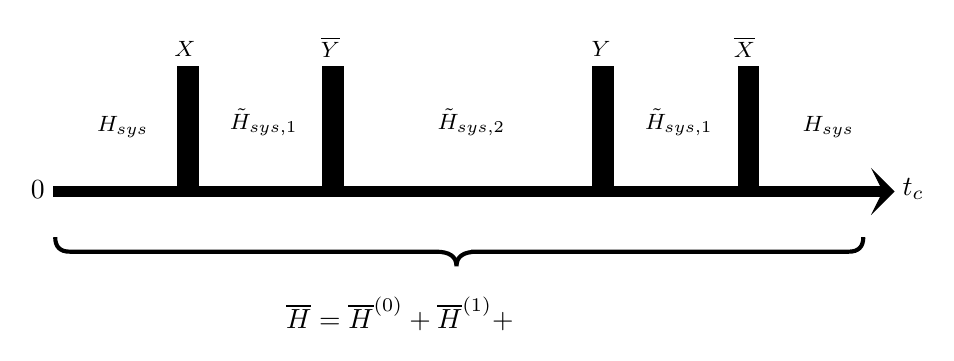
\begin{tikzpicture}[x=0.75pt,y=0.75pt,yscale=-1,xscale=1]
%uncomment if require: \path (0,327); %set diagram left start at 0, and has height of 327

%Shape: Rectangle [id:dp757529732417089]
\draw  [fill={rgb, 255:red, 0; green, 0; blue, 0 }  ,fill opacity=1 ] (80,60) -- (90,60) -- (90,120) -- (80,120) -- cycle ;
%Straight Lines [id:da8398663533091074]
\draw [line width=3.75]    (20,120) -- (420,120) ;
%Shape: Rectangle [id:dp8989097393091372]
\draw  [fill={rgb, 255:red, 0; green, 0; blue, 0 }  ,fill opacity=1 ] (150,60) -- (160,60) -- (160,120) -- (150,120) -- cycle ;
%Shape: Rectangle [id:dp5203891268410358]
\draw  [fill={rgb, 255:red, 0; green, 0; blue, 0 }  ,fill opacity=1 ] (280,60) -- (290,60) -- (290,120) -- (280,120) -- cycle ;
%Shape: Rectangle [id:dp5922766644502158]
\draw  [fill={rgb, 255:red, 0; green, 0; blue, 0 }  ,fill opacity=1 ] (350,60) -- (360,60) -- (360,120) -- (350,120) -- cycle ;
\draw  [fill={rgb, 255:red, 0; green, 0; blue, 0 }  ,fill opacity=1 ] (415,110) -- (425,120) -- (415,130) -- (420,120) -- cycle ;
%Shape: Brace [id:dp004729490444473794]
\draw  [line width=1.5]  (21,142) .. controls (21,146.67) and (23.33,149) .. (28,149) -- (204.33,149) .. controls (211,149) and (214.33,151.33) .. (214.33,156) .. controls (214.33,151.33) and (217.66,149) .. (224.33,149)(221.33,149) -- (403.33,149) .. controls (408,149) and (410.33,146.67) .. (410.33,142) ;

% Text Node
\draw (83.5,51.5) node  [font=\footnotesize] [align=left] {$\displaystyle X$};
% Text Node
\draw (153.5,50.5) node  [font=\footnotesize] [align=left] {$\displaystyle \overline{Y}$};
% Text Node
\draw (353,50.5) node  [font=\footnotesize] [align=left] {$\displaystyle \overline{X}$};
% Text Node
\draw (284,51.5) node  [font=\footnotesize] [align=left] {$\displaystyle Y$};
% Text Node
\draw (428,112.4) node [anchor=north west][inner sep=0.75pt]    {$t_{c}$};
% Text Node
\draw (8,113.4) node [anchor=north west][inner sep=0.75pt]    {$0$};
% Text Node
\draw (53.5,89) node  [font=\footnotesize]  {$H_{\text{sys}}$};
% Text Node
\draw (121.5,86.5) node  [font=\footnotesize]  {$\tilde{H}_{\text{sys, 1}}$};
% Text Node
\draw (221.5,86.5) node  [font=\footnotesize]  {$\tilde{H}_{\text{sys, 2}}$};
% Text Node
\draw (321.5,86.5) node  [font=\footnotesize]  {$\tilde{H}_{\text{sys, 1}}$};
% Text Node
\draw (393.5,89) node  [font=\footnotesize]  {$H_{\text{sys}}$};
% Text Node
\draw (131,169.4) node [anchor=north west][inner sep=0.75pt]    {$\overline{H} =\overline{H}^{( 0)} +\overline{H}^{( 1)} +\dotsc $};


\end{tikzpicture}
}

% \caption{}
% \label{}
\end{figure}


% For some pulse sequences with cycle time $t_c$, the time-evolution operator for one cycle can be given in terms of an average Hamiltonian
% \begin{equation*}
%     U(t_c) = \exp\left( -i t_c (\overline{H}^{(0)} +
%         \overline{H}^{(1)} + \dots) \right)
% \end{equation*}

\begin{align*}
    \overline{H}^{(0)} &= \frac{1}{t_c} \int_0^{t_c}
        \widetilde{H}_\text{system}(t) dt \\
    \overline{H}^{(1)} &= \frac{1}{2it_c} \int_0^{t_c} dt_1 \int_0^{t_1} dt_2
        [\widetilde{H}_\text{system}(t_1), \widetilde{H}_\text{system}(t_2)]
\end{align*}

\end{frame}

\begin{frame}{AHT (cont.)}

AHT has led to useful pulse sequences, but\dots
\begin{itemize}
    \item Typically only consider the lowest order term in average Hamiltonian (higher-order terms get tricky)
    \item Formalism is restrictive in identifying new, potentially better sequences
\end{itemize}

\end{frame}

\section{Reinforcement learning for quantum control}


\begin{frame}{Reinforcement learning for quantum control}

\begin{figure}
\centering
\includegraphics[width=.8\textwidth]{rl.png}
\caption{From \cite{sutton2018reinforcement}.}
\end{figure}

\begin{itemize}
    \item State $\to$ density operator or propagator
    \item Action $\to$ control Hamiltonian $H_\text{control}(t)$
    \item Reward $\to$ state or operator fidelity
\end{itemize}
    
\end{frame}

\begin{frame}{Reinforcement learning for quantum control (cont.)}

\begin{equation*}
    \text{fidelity}(U, U_\text{target}) = \Re{
        \frac{\Tr{U_\text{target}^\dagger U(t)}}{\Tr{\identity}}
    }
\end{equation*}
Generally use transformed version of fidelity for RL algorithms
\begin{equation*}
    r = -\log \left( 1 - \text{fidelity} \right)
\end{equation*}

Can apply RL to discrete control problem (pulse sequences)
or continuous control (shaped pulses, continuously-varying control
Hamiltonians)

\end{frame}

\begin{frame}{RL advantages and disadvantages}

\begin{itemize}
    \item Generalized approach to learning problem: no assumed prior knowledge
    \item Can tailor problem to specific system of interest (e.g. strongly coupled system, timing precision constraints)
    \item Robustness against known errors by including them in simulation of spin system
\end{itemize}

\pause

\begin{itemize}
    \color{red}
    \item Computationally expensive
    \item Poor accuracy of many-body spin simulations
    \item No guarantees for convergence to optimal (or good) solution
\end{itemize}

\end{frame}

\begin{frame}{Constructing pulse sequences using RL}

Implemented AlphaZero algorithm from \cite{Silver1140}.

\begin{figure}
\centering
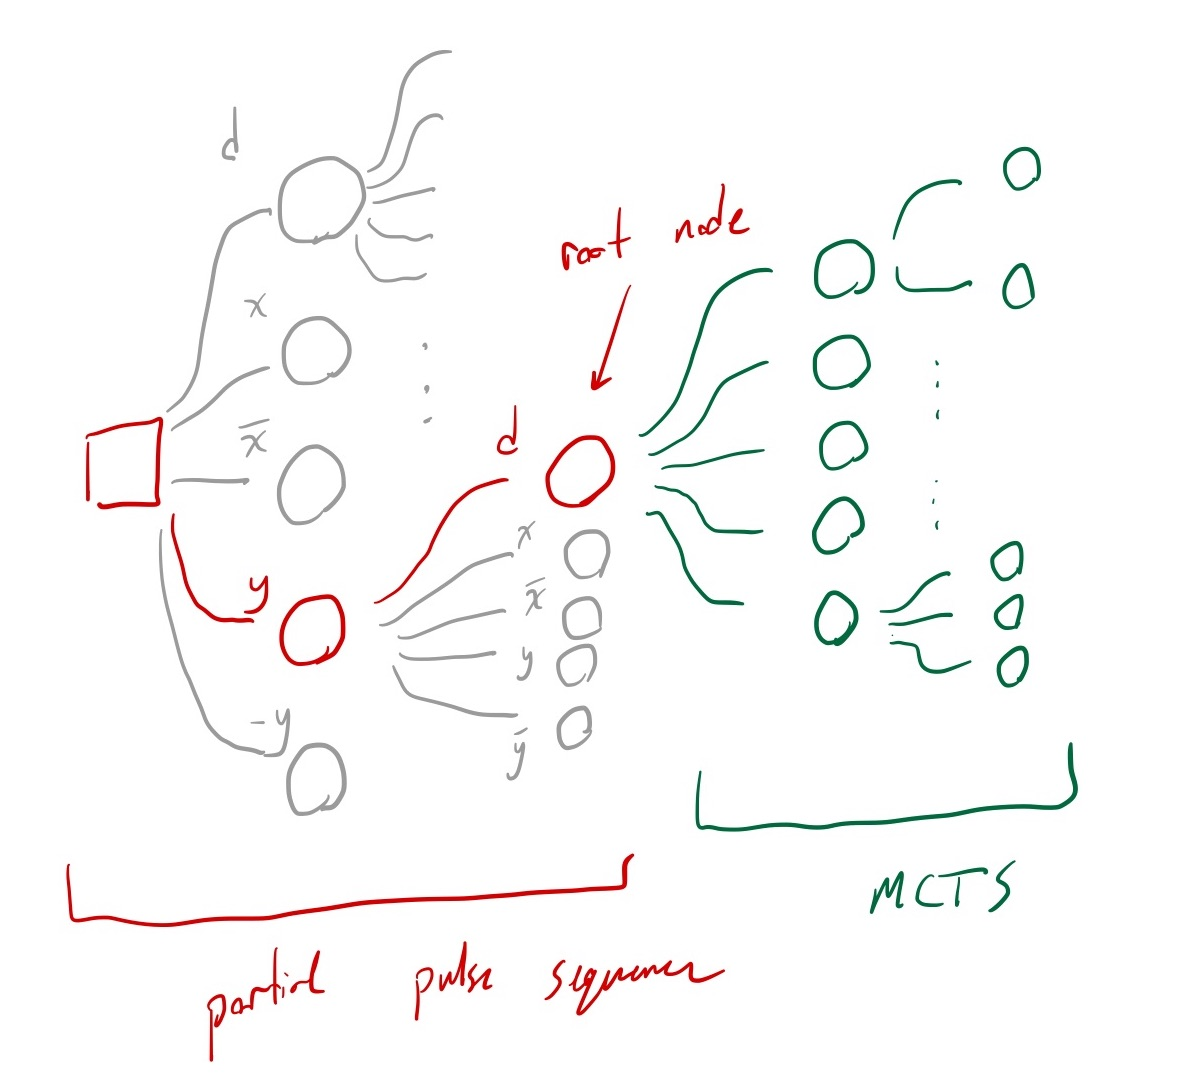
\includegraphics[width=.3\textwidth]{mcts.jpg}
% TODO add normal pulse sequence vizualization here...
\caption{Visualization of the AlphaZero algorithm and MCTS.
WORKING ON PULSE SEQUENCE VISUAL TO GO ALONG WITH ABOVE
}
\end{figure}



Collects data on pulse sequences, balancing \emph{exploration} of new
pulse sequences and \emph{exploitation} of learnings (via neural
networks), and trains neural networks on collected data to learn from
recent experiences.
\end{frame}

\begin{frame}{Computational results}

% TODO include results for weakly and strongly coupled spin systems

Searching for 48-pulse sequence for time suspension (\(\overline{H}=0\)) in strongly coupled spin system

\includegraphics[width=.49\textwidth]{rot_errors.png}
\includegraphics[width=.49\textwidth]{phase_transients.png}

AlphaZero algorithm ran on 16 Intel Xeon E5-2640V3 (2.6GHz) CPUs for 20+ hours.

\end{frame}

\begin{frame}{Experimental results}

\{decay plots, compare with yxx48 and CORY-48\}

waiting on results from (hopefully) better pulse sequence

\end{frame}

\begin{frame}[allowframebreaks]
\frametitle{References}

\printbibliography

\end{frame}

\section{Appendix}

\begin{frame}{Average Hamiltonian Theory (AHT)}

The time-evolution operator (or propagator) follows the differential
equation \[
i \frac{d}{dt} U(t) = H(t)U(t)
\] \[
U(0) = \identity
\]

The Magnus Expansion gives an exponential solution for the propagator
via an average Hamiltonian \(\overline{H}\) at time \(t\) \[
U(t) = \exp\left( -i \overline{H} t \right)
\] with \(\overline{H} = \overline{H}^0 + \overline{H}^1 + \dots\).

The series converges rapidly when \(t||H|| \ll 1\).

\end{frame}

\begin{frame}{AHT (cont.)}

We often work in the interaction frame of the control Hamiltonian, with transformation operator

\begin{align*}
    \frac{d}{dt} U_\text{control}(t) &=
        -i H_\text{control}(t)U_\text{control}(t) \\
    U_\text{control}(0) &= \identity
\end{align*}

So the Hamiltonian in the interaction frame becomes

\begin{equation*}
    \widetilde{H}(t) = \widetilde{H}_\text{system}(t) = U_\text{control}(t)^\dagger H_\text{system} U_\text{control}(t)
\end{equation*}

\cite{brinkmann_2016}.
\end{frame}

\begin{frame}{AHT: Pulse Sequences}

% TODO add density operator, diagrams

If a pulse sequence is both cyclic and periodic \cite{gerstein-dybowski}
\begin{align*}
    U_\text{control}(t_c) &= T\exp \left(
        -i \int_0^{t_c} H_\text{control}(t) dt \right) = \pm \identity
         \, \text{(cyclic)} \\
    H_\text{control}(t) &= H_\text{control}(t + Nt_c) \, \text{(periodic)}
\end{align*}
then the interaction frame and the lab frame coincide at multiples of
the cycle time, and the propagator can be given by
\begin{align*}
    U(t_c) &= \exp\left( -i t_c (\overline{H}^{(0)} +
        \overline{H}^{(1)} + \dots) \right) \\
    \overline{H}^{(0)} &= 1/t_c \int_0^{t_c}
        \widetilde{H}_\text{system}(t) dt \\
    \overline{H}^{(1)} &= 1/2it_c \int_0^{t_c} dt_1 \int_0^{t_1} dt_2
        [\widetilde{H}_\text{system}(t_1), \widetilde{H}_\text{system}(t_2)]
\end{align*}
Higher-order terms for average Hamiltonian become nasty.

\end{frame}

\begin{frame}{AHT: Special Cases}

\begin{itemize}

\item
  Symmetric pulse sequences (\(H(\tau) = H(t_c - \tau)\)): all odd-order
  terms in average Hamiltonian are zero
\item
  Antisymmetric pulse sequences (\(H(\tau) = - H(t_c - \tau)\)): all
  terms in average Hamiltonian are zero
\end{itemize}
\end{frame}

\begin{frame}{AHT: WHH-4 Example}

% TODO include Bloch sphere representation, or toggling frame changes

WORKING ON INTERACTION FRAME VISUAL, SHOWING HOW $I_z$ and $I_z I_z$ transform in interaction frame

\end{frame}

\begin{frame}{Reinforcement learning methodology}

% TODO fill in below

Working on this slide still...

State representation:

Action representation:

Spin system simulation parameters:

% TODO system/ensemble simulation

\end{frame}

\begin{frame}{Neural network structure}

Working on a better visual

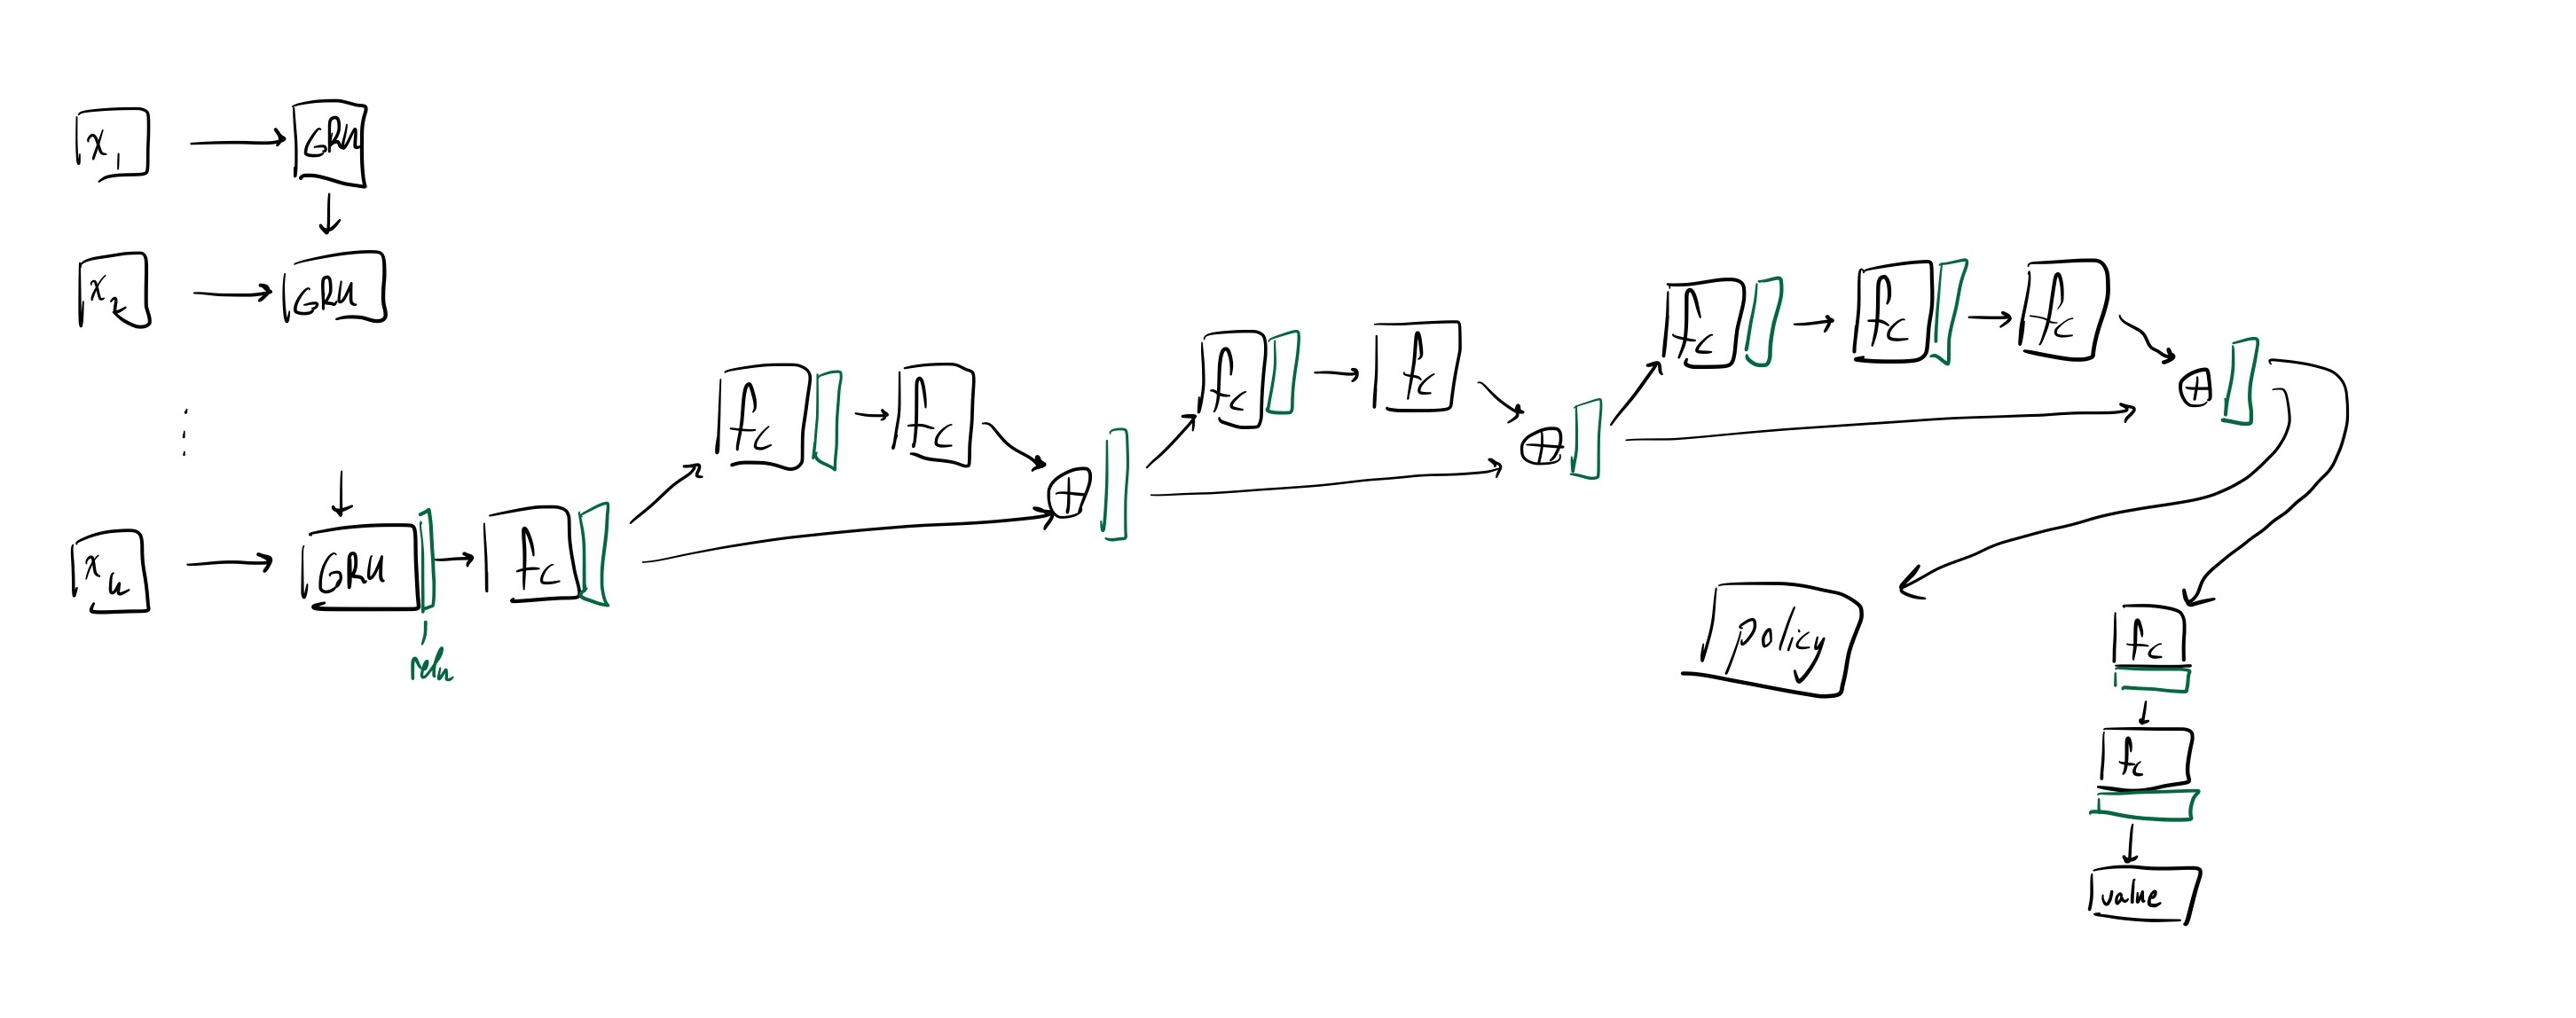
\includegraphics[width=.8\textwidth]{nn_structure.jpg}

\end{frame}

\begin{frame}{AlphaZero algorithm}

\begin{itemize}

\item
  Explore new pulse sequences

  \begin{enumerate}
  
  \item
    Start with a zero-length pulse sequence as the root node
  \item
    With the given root node, perform Monte Carlo Tree Search (MCTS) to
    explore potential pulses
  \end{enumerate}

  \begin{itemize}
  
  \item
    MCTS uses a neural network to estimate the prior probabilities for
    selecting each pulse and the value (fidelity) for the final pulse
    sequence
  \end{itemize}

  \begin{enumerate}
  \setcounter{enumi}{2}
  
  \item
    Sample the next pulse from the root node's children weighted by
    their visit counts
  \item
    Repeat steps 2-4 until a complete pulse sequence is determined
  \item
    Record the child nodes' visit counts and final pulse sequence
    fidelity to a data buffer for training
  \end{enumerate}
\item
  Train neural networks on collected data

  \begin{itemize}
  
  \item
    Policy loss: want to minimize the difference between MCTS visit
    counts \(\mathbf{p}\) and learned policy \(\pi_\theta\)
  \item
    Value loss: want to minimize the difference between calculated
    fidelity from pulse sequence \(z\) and predicted fidelity from
    neural network \(v\)
  \item
    L2 regularization: prevent overfitting to data
  \item
    \(l(\theta) = -\mathbf{p} \cdot \log\pi_\theta + (z - v)^2 + c||\theta||^2\)
  \end{itemize}
\end{itemize}

Parameters for MCTS, training, etc.
\end{frame}

\begin{frame}{Neural network training}

\includegraphics[width=.49\textwidth]{loss_policy.png}
\includegraphics[width=.49\textwidth]{loss_value.png}
\end{frame}

\begin{frame}{Training performance}

\includegraphics[width=.8\textwidth]{training_fidelity.png}
\end{frame}

\begin{frame}{Pulse sequences identified using AlphaZero}

\textrm{az48} pulse sequence (for time suspension):

$ -Y, \tau, -X, \tau, X, \tau, X, \tau, -X, \tau, X, \tau, -X, \tau, \tau_{\pi/2}, \tau $
$ -Y, \tau, \tau_{\pi/2}, \tau, Y, \tau, X, \tau, Y, \tau, -X, \tau, Y, \tau, \tau_{\pi/2}, \tau $
$ \tau_{\pi/2}, \tau, -X, \tau, -Y, \tau, -Y, \tau, -X, \tau, X, \tau, -X, \tau, -X, \tau $
$ -X, \tau, -Y, \tau, \tau_{\pi/2}, \tau, \tau_{\pi/2}, \tau, -X, \tau, Y, \tau, -Y, \tau, Y, \tau $
$ -Y, \tau, \tau_{\pi/2}, \tau, X, \tau, -Y, \tau, Y, \tau, X, \tau, Y, \tau, -Y, \tau $
$ \tau_{\pi/2}, \tau, \tau_{\pi/2}, \tau, -Y, \tau, \tau_{\pi/2}, \tau, -X, \tau, \tau_{\pi/2}, \tau, \tau_{\pi/2}, \tau, -Y, \tau $

\end{frame}


\end{document}
